% ---
% §1.1 Introducción. Reemplaza las líneas 476–569 de Docs/Technical_Report.tex.
% Se conserva la estructura de TT1 (contexto clínico, limitaciones de los métodos clásicos,
% computación cuántica) con las correcciones de la auditoría T3 (Docs/insumos/auditoria_s1_s2.md):
%   - GLOBOCAN se cita por la fuente primaria, Bray et al. (2024), no por Freihat et al. (2025);
%   - fuera Windsong Radiology (blog comercial) y Consultores Salud (fuente secundaria);
%   - \cite de Wang et al., Xiang et al. y Mari et al., que estaban parafraseados sin cita;
%   - fuera la atribución a Kim et al. (2025) de una frase sobre interpretabilidad que un artículo
%     epidemiológico difícilmente sostiene (pendiente de T9 #12);
%   - lenguaje calibrado: sin «fundamento de la ventaja cuántica», sin «correlaciones que los métodos
%     clásicos no capturan», sin «nuevos paradigmas que superen» lo clásico;
%   - erratas de TT1 corregidas (diagnóstivo, supervicencia, metastátis, embeddigs, etc.).
% Cifras verificadas contra la fuente en T9 (Docs/insumos/noche/informe_T9.md, 2026-10-16); las citas
% literales de cada párrafo están en sus comentarios % respaldo y pasan verificar_citas_fichas.py.
% Correcciones que salieron de T9: proyección a 2050 (+38 % y +68 %, Kim et al., no +50 % y +70 %);
% supervivencia en metástasis 33 % (no 30 %); Wang et al.: 6 modelos, 4 conjuntos y AUC de validación;
% tasa de México 15.7 → 18.7 (texto del INEGI); Kim et al. no habla de interpretabilidad (cita espuria);
% variabilidad entre lectores con Elmore et al. (1994); tamizaje con Monticciolo et al. (2021, ACR).
% ---

\subsection{Introducción}
\label{sec:introduccion}

\subsubsection{Contexto clínico del cáncer de mama}

El cáncer de mama es una enfermedad que se caracteriza por la proliferación descontrolada de células en el
tejido mamario, que forma tumores malignos con capacidad de propagarse si no reciben tratamiento
temprano. A nivel mundial es el cáncer diagnosticado con más frecuencia en las mujeres y la principal
causa de muerte por cáncer en ellas \cite{Bray2024GLOBOCAN}.

% respaldo: «Breast cancer and lung cancer were the most frequent cancers in women and men, respectively (both cases and deaths).» (Bray2024GLOBOCAN, p. 1)
% respaldo: «In 2022, breast cancer was diagnosed in 2.3 million women worldwide, resulting in 670,000 deaths.» (GLOBOCAN2022, p. 1)
% respaldo: «By 2050, new cases and deaths will have increased by 38% and 68%, respectively, disproportionately impacting low-HDI countries.» (Kim2025GlobalBreastCancer, p. 1)
Según las estimaciones de GLOBOCAN 2022 de la Agencia Internacional de Investigación sobre el Cáncer
(IARC), en 2022 se registraron alrededor de 2.3 millones de casos nuevos de cáncer de mama y unas
670\,000 defunciones en el mundo \cite{Bray2024GLOBOCAN, GLOBOCAN2022}. Para 2050 se proyecta que los
casos nuevos aumenten un 38\,\% y las defunciones un 68\,\%, con un impacto desproporcionado en los
países de menor índice de desarrollo humano \cite{Kim2025GlobalBreastCancer}.

Las diferencias regionales tienen implicaciones directas para el desarrollo de herramientas de
diagnóstico asistido. % respaldo: «Many low-income countries have high cancer mortality rates despite low cancer incidence, largely due to lack of or inadequate early detection and treatment services.» (GlobalCancerStatistics2024, p. 1)
En muchos países de bajos ingresos, la mortalidad por cáncer es alta pese a una incidencia baja, por
la falta de servicios de detección temprana y tratamiento oportuno: la mortalidad por cáncer de mama
es el doble en Etiopía que en Estados Unidos, con una incidencia un 60\,\% menor \cite{GlobalCancerStatistics2024}. El problema, por tanto, no es solo la frecuencia de la enfermedad, sino también la capacidad de los sistemas de salud para detectarla y tratarla a tiempo. Esto subraya la importancia de desarrollar herramientas que amplíen la capacidad diagnóstica, especialmente en regiones con recursos limitados.

\textbf{Panorama en México}

% respaldo: «En 2024, el cáncer de mama fue la primera causa de muerte entre los tumores malignos; 99.2 % ocurrieron en mujeres.» (INEGI2025, p. 1)
Según el Instituto Nacional de Estadística y Geografía (INEGI), en 2024 el cáncer de mama fue la primera causa de muerte por tumores malignos en México, con 8\,451 defunciones, el 99.2\,\% de ellas en mujeres, y una tasa de 18.7 por cada 100\,000 mujeres de 20 años o más
\cite{INEGI2025}. Durante la última década, esa tasa pasó de 15.7 en 2015 a 18.7 en 2024 (Figura~\ref{fig:MexicoBreastCancerStats}; la figura~\ref{fig:MexicoBreastCancerStatsByState} desglosa la incidencia y la mortalidad por entidad federativa).

% Figuras 1.1.1 y 1.1.2 — Incidencia y mortalidad por cáncer de mama en México
\begin{figure}[t]
  \begin{subfigure}[t]{0.48\textwidth}
    \centering
    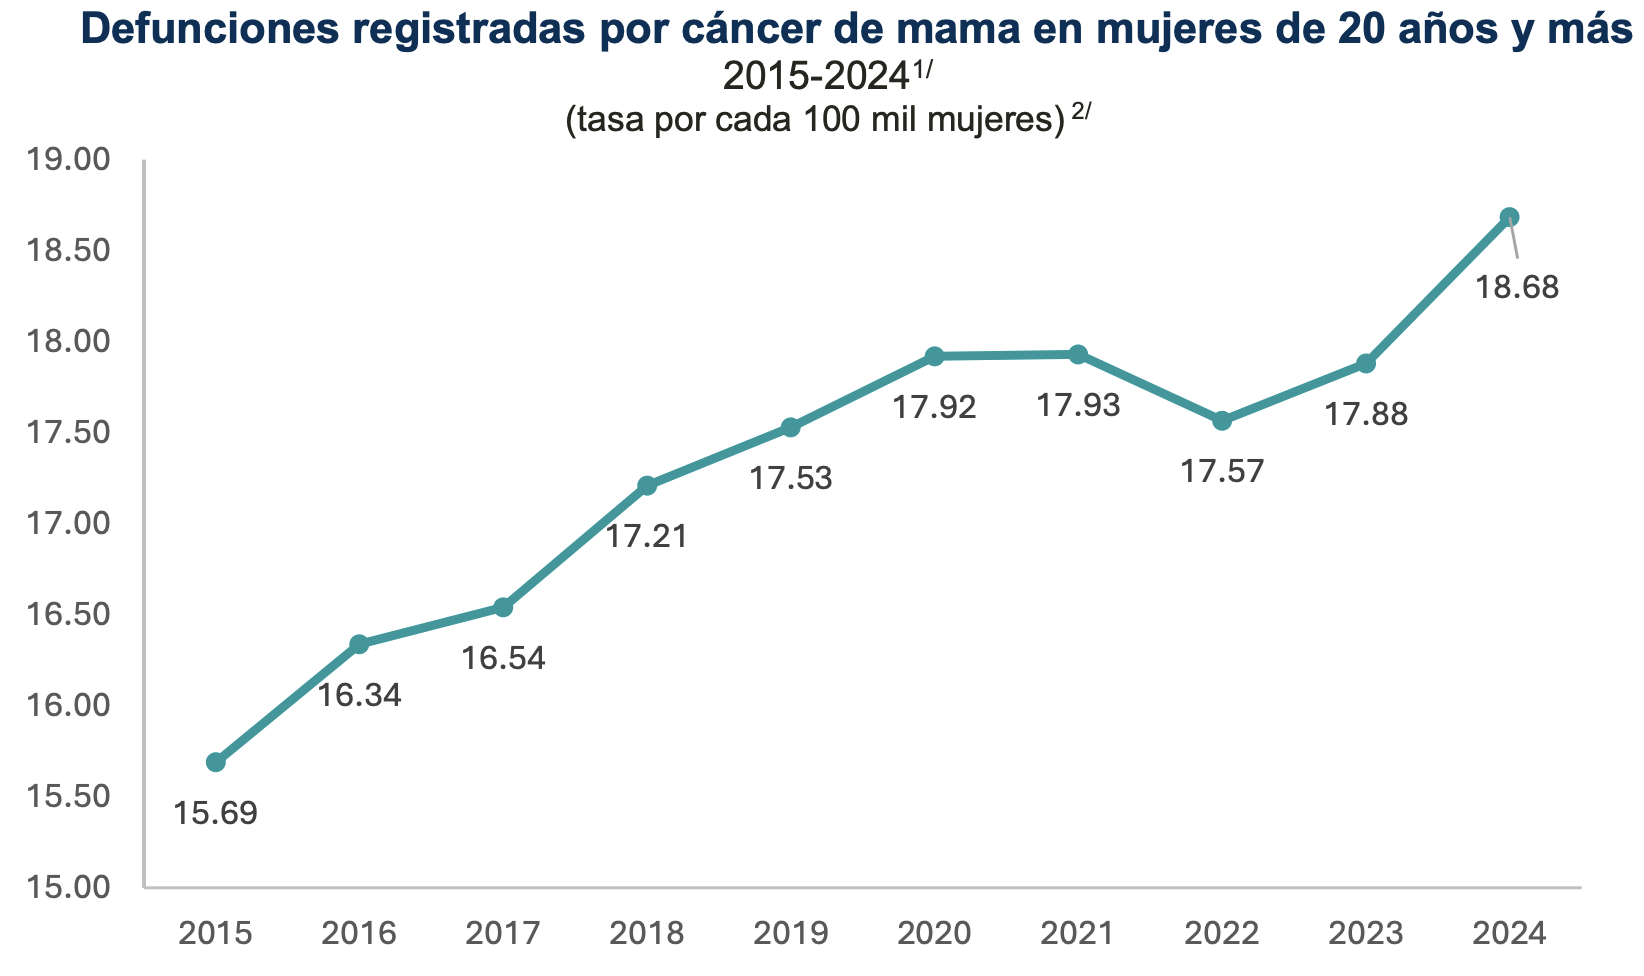
\includegraphics[width=\textwidth]{Figures/Figura_1_1_1.png}
    \caption{Tasa de mortalidad por cáncer de mama en México de 2015 a 2024 \cite{INEGI2025}.}
    \label{fig:MexicoBreastCancerStats}
  \end{subfigure}
  \hfill
  \begin{subfigure}[t]{0.48\textwidth}
    \centering
    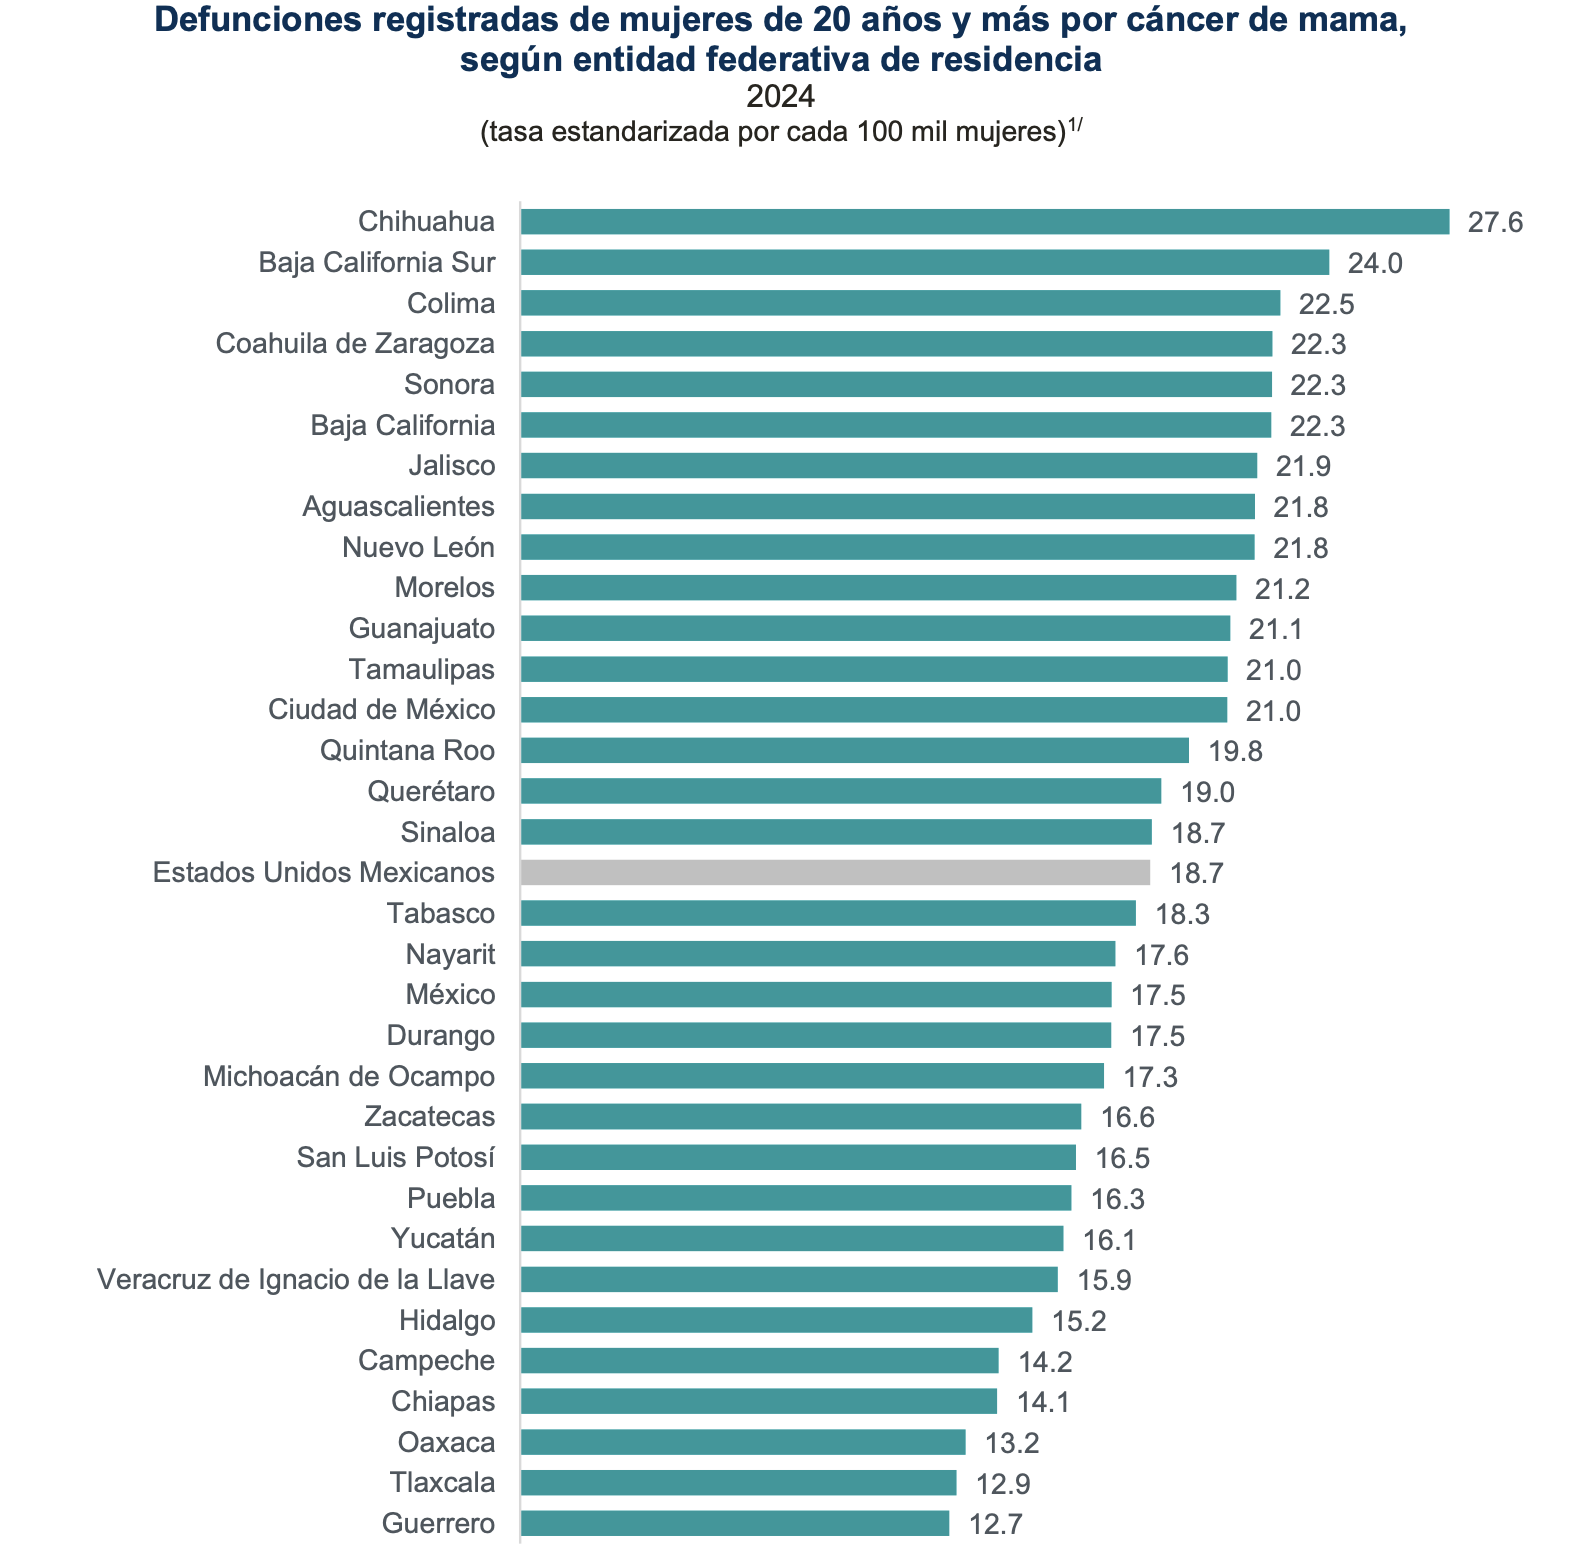
\includegraphics[width=\textwidth]{Figures/Figura_1_1_2.png}
    \caption{Incidencia y mortalidad por entidad federativa en México \cite{INEGI2025}.}
    \label{fig:MexicoBreastCancerStatsByState}
  \end{subfigure}
\end{figure}

\textbf{La detección temprana como factor determinante}

La detección temprana es el factor clínico que más justifica el desarrollo de sistemas de prediagnóstico.
% respaldo: «In fact, according to the American Cancer Society, the 5-year relative survival rate for breast cancer diagnosed at an early, localized stage is over 99%.» (NBCF2026_EarlyDetection, p. 1)
% dato: tabla «Breast Cancer (SEER*) Stage», fila «Distant … 33%» (Docs/fuentes/txt/NBCF2026_Facts/p001.txt, l. 311–313)
Según la American Cancer Society, cuando el cáncer de mama se detecta en una etapa temprana, la supervivencia relativa a cinco años supera el 99\,\%; con metástasis a distancia, según
los datos del programa SEER del National Cancer Institute, es del 33\,\%
\cite{NBCF2026_EarlyDetection, NBCF2026_Facts}.

% respaldo: «Mammography screening has been proven effective in reducing breast cancer deaths in women age 40 years and older. A mortality reduction of 40% is possible with regular screening.» (Monticciolo2021ACR, p. 1)
% respaldo: «radiologists can differ, sometimes substantially, in their interpretations of mammograms and in their recommendations for management.» (Elmore1994, p. 1)
La mamografía es el instrumento central de la detección temprana: el American College of Radiology
señala que el tamizaje mamográfico reduce las muertes por cáncer de mama en mujeres de 40 años o más,
y que con un tamizaje regular es posible una reducción de la mortalidad del 40\,\%
\cite{Monticciolo2021ACR}. Sin embargo, su interpretación manual tiene limitaciones. Los radiólogos
pueden diferir, a veces de forma sustancial, en su interpretación de una misma mamografía y en la
conducta que recomiendan \cite{Elmore1994}; a ello se suman la dificultad de detectar lesiones en tejido
mamario denso y la carga de trabajo creciente de los sistemas de salud. Estos factores
motivan el desarrollo de sistemas de diagnóstico asistido por computadora (CADx).

En México, la infraestructura diagnóstica sigue siendo un desafío. En 2021 se registraron 1\,281
mastógrafos en el país: el 41.1\,\% en instituciones de salud y seguridad social, el 36.1\,\% en
establecimientos particulares y el 22.8\,\% en servicios para población sin derechohabiencia
\cite{INEGI2023}. Esta distribución, junto con el aumento sostenido de la
mortalidad, marca la necesidad de herramientas que amplíen la capacidad diagnóstica del sistema de salud.

En este contexto, el presente trabajo explora el uso de transformaciones cuánticas variacionales
sobre características extraídas de mamografías del dataset CBIS-DDSM, con el fin de evaluar en qué
medida estas representaciones modifican la separación de las clases benigna y maligna cuando se
integran como entrada de una red neuronal clásica.

\subsubsection{Limitaciones de los métodos clásicos de diagnóstico asistido}

El diagnóstico asistido por computadora en mamografía se ha desarrollado notablemente en las últimas
dos décadas, impulsado por las redes neuronales convolucionales (CNN) y el aprendizaje profundo
\cite{TandFOnline2021}. Pese a los resultados reportados en condiciones controladas, estos métodos
presentan limitaciones que restringen su aplicación clínica generalizada.

\textbf{Variabilidad entre conjuntos de datos}

Los modelos de aprendizaje profundo no eliminan la inconsistencia de la interpretación humana: la
trasladan a otro plano. En lugar de variar entre observadores, su desempeño varía entre conjuntos de
% respaldo: «Six deep learning models (three published models with high performance and three models designed by us) were evaluated on four different mammogram data sets» (Wang2020DeepLearning, p. 1)
% respaldo: «However, the same evaluation criteria of all six models on the three external test data sets were significantly decreased, only between 0.44 (95% CI: 0.43-0.45) and 0.65 (95% CI: 0.64-0.66).» (Wang2020DeepLearning, p. 1)
% respaldo: «The three published models reported validation auROC scores between 0.88 and 0.95 on the validation data set.» (Wang2020DeepLearning, p. 1)
datos. Wang et al. \cite{Wang2020DeepLearning} evaluaron seis modelos de aprendizaje profundo, tres
publicados con alto desempeño y tres propios, sobre cuatro conjuntos de mamografías. Los tres modelos
publicados reportaban un AUC-ROC de validación de entre 0.88 y 0.95; sobre los tres conjuntos de
prueba externos, los seis modelos obtuvieron valores de apenas entre 0.44 y 0.65. Un alto desempeño de un sistema CADx en el conjunto de datos con el que se desarrolló no garantiza la
misma efectividad en datos con otra distribución, condición inevitable en la práctica clínica, donde los equipos de adquisición, las
poblaciones y los protocolos de imagen varían.

\textbf{Interpretabilidad}

% Argumento de diseño propio, sin cita (decidido por el autor el 2026-10-16). La cita a Kim et al.
% (2025) de TT1 se retiró: es un artículo epidemiológico que no trata la interpretabilidad (T9 #12).
Una red convolucional profunda aprende sus propias representaciones internas de la imagen, que no
tienen un significado clínico directo. Este trabajo usa, en cambio, características radiómicas, cuyo
significado es explícito: cada una mide una propiedad definida de la intensidad, la textura o la
forma de la lesión. Así es posible saber qué información recibe cada representación y, por tanto,
interpretar qué cambia cuando se le aplica una transformación cuántica.

\textbf{Dimensionalidad y tamaño de los datos}

Las imágenes mamográficas tienen una dimensionalidad muy alta en relación con el número de casos
disponibles. Cuando el conjunto de entrenamiento es pequeño frente al número de parámetros de un
modelo, este tiende a sobreajustarse: aprende los detalles de los datos de entrenamiento y no
generaliza a datos nuevos. El aumento de datos y la regularización mitigan el problema sin
resolverlo, especialmente en conjuntos de tamaño moderado como el CBIS-DDSM.

Estas limitaciones motivan la búsqueda de representaciones alternativas de los datos, entre ellas
las cuánticas, y la evaluación rigurosa de si aportan algo a la separabilidad de las clases.

\subsubsection{Computación cuántica como alternativa}

La computación cuántica ofrece mecanismos distintos para representar y transformar datos. En el
aprendizaje automático, su propuesta no es sustituir a los métodos clásicos, sino intervenir en etapas
específicas del procesamiento, en particular en la codificación de las características.

\textbf{El espacio de Hilbert como espacio de representación}

Un circuito de codificación $U(\mathbf{x})$ define un mapeo no lineal
$\phi: \mathbb{R}^n \rightarrow \mathcal{H}$ que lleva un vector de características clásico
$\mathbf{x}$ a un estado cuántico $|\phi(\mathbf{x})\rangle$ del espacio de Hilbert $\mathcal{H}$. La
geometría de ese espacio la determinan las fidelidades
$|\langle\phi(\mathbf{x})|\phi(\mathbf{x}')\rangle|^2$ entre estados, y no las distancias euclidianas
entre vectores, y depende directamente del diseño del circuito. Cuando el circuito entrelaza los
qubits, la representación puede incorporar dependencias entre pares de características
(sección~\ref{sec:feature_map}). Si esa geometría resulta más favorable para separar lesiones
benignas y malignas que las representaciones clásicas es una pregunta empírica, y es el objeto de
estudio de este trabajo (sección~\ref{sec:planteamiento}).

\textbf{Modelos híbridos cuántico-clásicos para el diagnóstico}

% respaldo: «In this work, we present a quantum hybrid classical convolutional neural network (QCCNN) based breast cancer diagnosis approach with the goal of utilizing quantum computing’s high-dimensional data processing power and parallelism to increase diagnosis efficiency and accuracy.» (Xiang2024QuantumCNN, p. 1)
% respaldo: «The full network is a map from a classical vector space to a classical vector space depending on classical weights.» (Mari2020Transfer, p. 3)
La aplicación del aprendizaje automático cuántico al diagnóstico clínico es una línea de
investigación activa, en la que predominan las arquitecturas híbridas: los circuitos cuánticos se
integran como componentes especializados dentro de un procesamiento mayoritariamente clásico. Xiang
et al. \cite{Xiang2024QuantumCNN} proponen, por ejemplo, una red convolucional híbrida para el
diagnóstico de cáncer de mama con el objetivo de aprovechar el procesamiento de datos de alta
dimensión de la computación cuántica. Mari et al. \cite{Mari2020Transfer} formalizan este tipo de
modelos: la red completa, incluida la capa de codificación cuántica y la medición final, es una
función de un espacio vectorial clásico a otro que depende de pesos clásicos y que, vista desde
fuera, es análoga a una red clásica profunda. Este trabajo usa el circuito de la misma manera, como
una transformación entre representaciones clásicas, pero sin entrenarlo: sus parámetros se fijan para
poder medir su efecto sobre la separabilidad de forma aislada.

\textbf{Estado actual y expectativas}

% respaldo: «We find that overall, out-of-the-box classical machine learning models outperform the quantum classifiers.» (Bowles2024Benchmarking, p. 1)
% respaldo: «Moreover, removing entanglement from a quantum model often results in as good or better performance, suggesting that “quantumness” may not be the crucial ingredient for the small learning tasks considered here.» (Bowles2024Benchmarking, p. 1)
El campo se encuentra en una etapa temprana. En un estudio comparativo a gran escala, Bowles et al.
\cite{Bowles2024Benchmarking} encontraron que, en conjunto, los modelos clásicos estándar, sin ajustes
especiales, superan a los clasificadores cuánticos en las tareas pequeñas que evaluaron, y que eliminar el
entrelazamiento de un modelo cuántico a menudo da un desempeño igual o mejor. Con los dispositivos y
simuladores disponibles no es posible aún demostrar con métricas concluyentes una ventaja de los
modelos cuánticos en problemas prácticos. El valor de una investigación como esta reside en explorar
y documentar, con un protocolo riguroso, sus posibilidades y sus limitaciones en un dominio de alto
impacto como el diagnóstico de cáncer de mama.
